\chapter{Estado del Arte}

\section{Información previa a considerar}

Para entrar de lleno en la tema, es necesario conocer de antemano varios aspectos básicos de la biología.

\subsection{Biomoléculas}

Cada vez que se habla de la biología, este concepto se relaciona directamente con la ciencia que estudia a los seres vivos. Ahora bien, las estructuras o compuestos que constituyen una parte esencial de los seres vivos son conocidas como \textbf{biomoléculas}. Estas biomoléculas están principalmente constituidas por elementos químicos como el carbono (C), hidrógeno (H), oxígeno (O), nitrógeno (N), fósforo (P) y azufre (S) \cite{biomolecula} y se pueden clasificar en biomoléculas inorgánicas, que se encuentran tanto en seres vivos como en los cuerpos inertes, no obstante son imprescindibles para la vida; y las biomoléculas orgánicas, que son sintetizadas por los seres vivos y tienen una estructura en base a carbono. Estas biomoléculas orgánicas se pueden separar en 4 grandes grupos:
\begin{enumerate}
\item Glúcidos (hidratos de carbono o carbohidratos): son la fuente de energía primaria que utilizan los seres vivos para realizar sus funciones vitales. Los ejemplos más conocidos son la glucosa, el almidón y el glucógeno.
\item Lípidos: conforman el principal almacén de energía de los animales y desempeñan funciones reguladores de enzimas y hormonas.
\item Ácidos nucleicos: El ácido desoxirribonucleico y el ácido ribonucleico, mayormente conocidos como ADN (DNA) y ARN (RNA y sus derivados) desarrollan posiblemente la función más importante para la vida: contener, de manera codificada, las instrucciones necesarias para el desarrollo y funcionamiento de la célula. El ADN tiene la capacidad de replicarse, transmitiendo así dichas instrucciones a las células hijas que heredarán la información.
\item Proteínas: poseen la mayor diversidad de funciones que realizan en los seres vivos; prácticamente todos los procesos biológicos dependen de su presencia y/o actividad. Son proteínas casi todas las enzimas, catalizadores de reacciones metabólicas, hemoglobina, anticuerpos, entre otros. Su unidad base es el {\it{aminoácido}}, por el cual se van formando los péptidos según la cantidad de unidades bases enlazadas.
\end{enumerate}

Dentro de estas biomoléculas, el análisis detallado de los carbohidratos y los lípidos depende en demasía de su estructura química (elementos químicos asociados y tipo de enlaces entre ellos), por lo mismo es una materia más ligada a los químicos (ver Figura 2.1). 

\begin{figure}[H] 

\begin{subfigure}{0.5\textwidth}
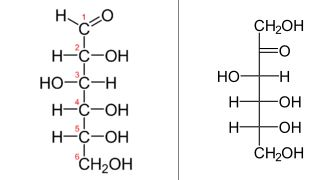
\includegraphics[width=0.9\linewidth, height=5cm]{./images/glucidoejemplos} 
\caption{Glúcidos (glucosa y fructosa).}
\label{fig:subim1}
\end{subfigure}
\begin{subfigure}{0.4\textwidth}
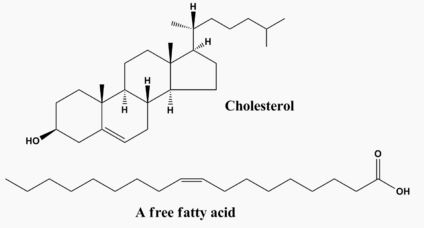
\includegraphics[width=1\linewidth, height=5cm]{./images/lipidosejemplos}
\caption{Lípidos (colesterol y un ácido graso).}
\label{fig:subim2}
\end{subfigure}
 
\caption{Estructura química de los carbohidratos y lípidos.}
\label{fig:image1}
\end{figure}

Sin embargo, el ADN y los polipéptidos poseen unidades base que pueden ser codificadas como letras, por consiguiente pueden ser secuenciados como {\it{cadenas de strings}} y en donde los avances computacionales y la evolución informática toman una importante relevancia (ver Figura 2.2).

\begin{figure}[H]

\begin{subfigure}{0.5\textwidth}
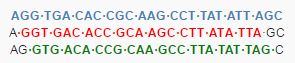
\includegraphics[width=1\linewidth, height=2cm]{./images/adnejemplo}
\caption{Cadena de ADN aleatoria.}
\label{fig:subim4}
\end{subfigure}
\begin{subfigure}{0.4\textwidth}
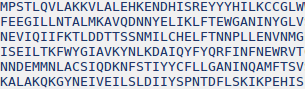
\includegraphics[width=1\linewidth, height=3cm]{./images/cadenaproteina} 
\caption{Cadena aleatoria de una proteína.}
\label{fig:subim3}
\end{subfigure}
 
\caption{Biomoléculas de ADN y péptidos llevadas a cadenas de strings.}
\label{fig:image2}
\end{figure}

Con respecto a estas 2 últimas estructuras, la diferencia visual más notoria radica en la cantidad de diferentes letras (strings) que las componen, para el ADN son 4 [8] y son denominadas \textbf{bases nitrogenadas} que son las siguientes:

\begin{enumerate}
\item Adenina
\item Timina
\item Citosina
\item Guanina
\end{enumerate}

Para las proteínas, su elemento básico como ya se mencionó anteriormente es el \textbf{aminoácido}, y ahora se adentrará en más detalle sobre esta molécula.

\subsection{Aminoácidos}

Los aminoácidos tienen diferentes funciones en el organismo \cite{amino} pero ante todo sirven como \textbf{las unidades básicas de los péptidos y de las proteínas.} A nivel orgánico el aminoácido es una molécula compuesta con un grupo amino (-NH2) y un grupo carboxilo (-COOH) y que pueden tener distintas distribuciones. Para el caso de los que componen las proteínas se consideran como alfa-aminoácidos:

\begin{figure}[h]
    \centering
    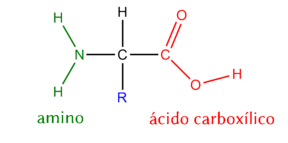
\includegraphics[width=0.4\textwidth]{./images/aminoacido}
    \caption{Estructura general de un alfa-aminoácido.}
    \label{fig:image3}
\end{figure}

En la imagen anterior se puede identificar el carbono central (alfa) unido al grupo carboxilo (rojo), grupo amino (verde), un hidrógeno (imagen superior color negro) y el grupo radical (azul) o R. Este grupo radical es el que determina la identidad y las propiedades de cada uno de los diferentes aminoácidos.

El primer aminoácido fue descubierto a principios del siglo XIX, y a partir de ese entonces hasta la actualidad son miles los aminoácidos que han sido descubiertos, pero solo 20 se consideran como los componentes esenciales para las proteínas (y los que se considerarán como parte de esta memoria) que se presentarán a continuación en conjunto con su respectiva abreviación utilizada en las cadenas de proteínas de los archivos FASTA \cite{fasta}:

\begin{table}[H]
\centering
\label{my-label5}
\begin{tabular}{|l l l l|}
\hline
\multicolumn{4}{|c|}{Aminoácido - Abreviatura}\\ \hline
Alanina - A      & Cisteína - C       &      Ácido aspártico - D     & Ácido glutámico - E                     \\
Fenilalalina - F      &  Glicina - G           & Histidina - H     & Isoleucina - I                \\
Lisina - K      & Leucina - L            & Metionina - M           & Aspargarina - N          \\
Prolina - P      & Glutamina - Q          & Arginina - R                  & Serina - S                  \\
Treonina - T      & Valina - V          & Triptófano - W                      & Tirosina - Y   \\ \hline
\end{tabular}
\caption{Los 20 aminoácidos existentes y considerados.}
\end{table}

Existen otras abreviaturas en las cadenas como B, X o J, pero para el alcance de esta memoria no serán considerados como objeto de estudio y análisis posterior.

A partir de este pequeño elemento se forman las macromoléculas que se identifican según la cantidad de aminoácidos (a partir de ahora se mencionarán como aa.) que los compongan \cite{array}:

\begin{table}[H]
\centering
\label{my-label1}
\begin{tabular}{|c|c|}
\hline
Tamaño & \multicolumn{1}{c|}{Tipo de estructura}  \\ \hline
Entre 2 y 14 aa.      &      Oligopéptido                             \\
Entre 15 y 50 aa.      &   Polipéptido      \\
Mayor de 50 aa.   &   Proteína            \\ \hline
\end{tabular}
\caption{Identificación de macromoléculas según cantidad de aminoácidos.}
\end{table}

El concepto de péptido \cite{array} hace referencia a aquellos elementos que contienen un enlace peptídico (2 aminoácidos se unen por medio de este tipo de enlace). Los prefijos \textit{oligo} y \textit{poli} provienen del griego $o \lambda \iota \gamma o$ (no demasiados) y $\pi o \lambda \upsilon$ (demasiados).

\section{Secuencias de proteínas}

Desde el momento en que se descubrieron los elementos componentes del ADN y las proteínas, se han investigado sobre las posibles combinaciones que se pueden encontrar entre las bases que los conforman y en qué cantidad se encuentran. Para el ADN y sus 4 elementos básicos existen millones de seres vivos, parásitos, virus, protozoos y entre otros que se definen por su código genético, por lo cual es posible encontrar los diversos residuos de bases según un determinado tamaño. En el caso puntual para la finalidad de este escrito y según lo mencionado por \cite{zamyatnin1}, es posible estudiar de manera teórica y con fórmulas matemáticas la cantidad máxima de fragmentos que puede formar una proteína. Considerando como base que el número posible de estructuras peptídicas naturales $P$ están compuestas de diferentes residuos de aminoácidos (incluyendo repeticiones en cadenas de aminoácidos) sigue la siguiente fórmula:

\begin{equation}
P=A^{n}
\end{equation}

Donde $A$ es el número de diferentes aminoácidos existentes, y $n$ es la cantidad de aminácidos correspondientes a la estructura estudiada. Por lo mismo y siguiendo esta fórmula (considerando $A=20$) la cantidad de diferentes combinaciones péptidos de tamaño $k$ que se pueden obtener se aprecian en la siguiente Tabla:

\begin{table}[H]
\centering
\label{my-label2}
\begin{tabular}{|c|c|}
\hline
Tamaño péptido (k) & \multicolumn{1}{c|}{Combinaciones posibles ($A^{k}$)}  \\ \hline
2 aa.     & 400        \\
3 aa.     & 8000                         \\
4 aa.      &      160000                             \\
5 aa.      &   3200000       \\
10 aa.      &   1.024$\times 10^{13}$       \\
20 aa.      &   1.049$\times 10^{26}$       \\
50 aa.   &     1.126$\times 10^{65}$   \\ \hline
\end{tabular}
\caption{Combinaciones posibles a obtener según el tamaño del péptido.}
\end{table}

Según lo observado en esta Tabla se identificar que a medida que el valor de $k$ va en aumento, las posibles combinaciones que se pueden obtener de fragmentos de proteínas pueden llegar a tener valores inimaginables para el ser humano corriente; no obstante, no todas estas estructuras existen o son capaces de ser encontradas en la naturaleza \cite{array}, aun así la diversidad de la búsqueda de estos residuos sigue siendo gigantesca, y por ende difícil de solucionar, y este será uno de los problemas que se intentará solucionar en esta memoria.

Ahora bien, para un polipéptido con un tamaño de $n$ aminoácidos, el máximo número posible de fragmentos de tamaño $k$ que teóricamente se podrían obtener (considerando las posibles repeticiones de fragmentos) es descrita mediante la siguiente expresión:

\begin{equation}
N_{k}^{teorica}=n-k+1
\end{equation}

Por consecuencia, el máximo número posible de fragmentos (con repeticiones) que teóricamente se pueden obtener para una molécula de tamaño $n$, partiendo desde $k=2$ (dipéptidos) hasta $k=n-1$, viene dado por:

\begin{equation}
N_{max}^{teorica}=\sum_{2}^{n-1} \frac{k(k-1)}{2}-1
\end{equation}

Mediante estas fórmulas, se han calculado la cantidad de posibles fragmentos que se pueden obtener en diferentes oligopéptidos y proteínas:

\begin{table}[H]
\centering
\label{my-label3}
\begin{tabular}{|c|l|r|r|}
\hline
Número & \multicolumn{1}{c|}{Oligopéptido/Proteína} & \multicolumn{1}{c|}{$n$} & \multicolumn{1}{c|}{$N_{suma}^{teorica}$} \\ \hline
1      & Encefalina (varios tipos biológicos)       & 5                        & 9                     \\
2      & Bradiquinina (mamíferos)                   & 9                        & 35                    \\
3      & ACTH (humanos)                             & 39                       & 740                   \\
4      & Cadena $\alpha$ hemoglobina (humanos)          & 141                      & 9869                  \\
5      & Cadena $\beta$ hemoglobina (humanos)          & 146                      & 10584                 \\ \hline
\end{tabular}
\caption{Número máximo posible de fragmentos que se pueden formar en 3 oligopéptidos (números 1, 2 y 3) y 2 proteínas (números 4 y 5).}
\end{table}

Considerando que para un polipéptido cuyo largo es de $n$ aminoácidos, si este valor de $n$ es muy alto, se puede obtener una cantidad muy alta de fragmentos de dipéptidos, pero muchos de estos dipéptidos se pueden repetir varias veces en la cadena, por lo tanto, cuando se desea obtener {\bf{el máximo número de fragmentos diferentes}} asociado a un valor $k$ determinado, este puede tener un valor muy bajo en comparación con la cantidad total de fragmentos obtenidos. Por medio de las fórmulas descritas anteriormente, se puede obtener el número máximo de diferentes fragmentos (o fragmentos esperables) asociado a un tamaño $k$:

\begin{equation}
N_{k}^{diff}=N_{k}^{teorica}- R_{k}
\end{equation}

Este valor $R_{k}$, se obtiene introduciendo nuevos parámetros $i$ (que es el número de estructuras idénticas para determinado $k$) y $m$ (el número de diferentes estructuras para el determinado $k$):

\begin{equation}
R_{k}=\sum_{1}^{m}(i-1)
\end{equation}

Por lo tanto, el número máximo de fragmentos diferentes que se pueden obtener en una proteína sigue la siguiente fórmula:

\begin{equation}
N_{max}^{diff}=\Bigg[\sum_{2}^{n-1} \frac{k(k-1)}{2}-1\Bigg]- \sum_{2}^{n-1}\Bigg[\sum_{1}^{m}(i-1)\Bigg]
\end{equation}
\\
Tomando la información de la base de datos de oligopéptidos EROP-Moscow, para mostrar los valores obtenidos con estas fórmulas, se usará como ejemplo la caseína bovina (proteína proveniente de la vaca). Esta proteína se compone de 4 subunidades, $\alpha - s1$, $\alpha -s2$, $\beta$ y $\kappa$. La siguiente Tabla muestra las cantidades teóricas y diferentes de fragmentos obtenidos como dipéptidos y sus sumas totales:

\begin{table}[H]
\centering
\label{my-label4}
\begin{tabular}{|c|l|c|c|c|c|c|}
\hline
Número & \multicolumn{1}{c|}{Caseína bovina (subunidad)} & $n$ & $N_{2}^{teorica}$ & \multicolumn{1}{l|}{$N_{2}^{diff}$} & \multicolumn{1}{l|}{$N_{max}^{teorica}$} & \multicolumn{1}{l|}{$N_{max}^{diff}$} \\ \hline
1      & $\alpha - s1$                                   & 199 & 198               & 134                                 & 19700                                     & 19621                                  \\
2      & $\alpha - s2$                                   & 207 & 206               & 131                                 & 21320                                     & 21216                                  \\
3      & $\beta$                                         & 209 & 208               & 124                                 & 21735                                     & 21641                                  \\
4      & $\kappa$                                        & 169 & 168               & 118                                 & 14195                                     & 14138                                  \\
5      & $\alpha - s1 + \alpha - s2 + \beta + \kappa$    & 784 & 780               & 260                                 & 76950                                     & 76304                                  \\ \hline
\end{tabular}
\caption{Número máximo posible de fragmentos que se pueden obtener en una proteína de caseína bovina.}
\end{table}

Se puede identificar que para los fragmentos de dipéptidos, la cantidad de diferentes fragmentos es bastante menor que la cantidad total de fragmentos obtenidos para las 4 subunidades, pero aún así la cantidad de fragmentos diferentes totales obtenidos es prácticamente la misma que la cantidad de fragmentos totales sin diferenciar. Esto es notorio ya que si $k$ va en progresivo aumento, el universo combinatorio de posibles fragmentos formados se acorta drásticamente, lo que también favorece a la baja formación de fragmentos que se repiten.

\section{Bases de datos de proteínas}

Estas bases de datos contienen proteínas expresadas como cadenas de texto y se diferencian según a la cantidad total que poseen. Las bases de datos usadas son 4:

\begin{table}[h]
\centering
\begin{tabular}{|l|c|c|c|}
\hline
\multicolumn{1}{|c|}{\textbf{Bases de datos}} & \textbf{Proteínas} & \textbf{Tamaño (MB)} & \textbf{Tamaño cadena (MB)} \\ \hline
SwissProt    & 555.426                & 268,3                & 199,5              \\
TrEMBL        & 89.396.316              & 40.900      & 30.200   \\
EROP-Moscow        & 14.785                 & 1,5                  & 0,3526                \\
Proteínas humanas     & 86.298                 & 47,2                 & 38,2               \\ \hline
\end{tabular}
\caption{\textit{Datasets} utilizados para la obtención de los resultados.}
\label{tb:labelea1}
\end{table} 

\subsection{Base de datos UniProt}

UniProt (nombre que proviene de \textit{\textbf{Uni}versal \textbf{Prot}ein}) es una base de datos de secuencias de proteínas e información funcional respectiva. Su fuente de investigación la compone un consorcio cuyos participantes son el Instituto Europeo de Bioinformática (EBI - \textit{European Bioinformatics Institute}), el Instituto Suizo de Bioinformática (SIB - \textit{Swiss Institute of Bioinformatics}) y los Recursos de Información de Proteínas (PIR - \textit{Protein Information Resource}) quienes compusieron UniProt en Diciembre del 2003. Cada uno de estos consorcios está altamente envuelto en las anotaciones y mantenimiento de las bases de datos que corresponden a UniProt, gracias a eso nace \textbf{UniProtKB} (UniProt Knowledgebase), que es una base de datos de proteínas comisariada por expertos, que se compone de 2 secciones:


\begin{enumerate}

\item \textbf{UniProt - SwissProt}: es una base de datos de secuencias de proteínas manualmente anotadas y revisadas. Combina información extraída de la literatura científica y un posterior análisis computacional. Está compuesto de 555.426 secuencias de proteínas que equivalen a un texto con un peso de 268 MB.

\item \textbf{UniProt - TrEMBL}: es una base de datos de secuencias de proteínas automáticamente anotadas y no revisadas. Estas secuencias son registros de alta calidad y computacionalmente analizados. Esta base de datos fue introducida en respuesta para aumentar el flujo de datos que se obtienen de los proyectos relacionados al genoma. Por está compuesto por 89.396.316 secuencias de proteínas que equivalen a un texto con un peso de 40 GB.

\item \textbf{Proteínas Humanas}: es una base de datos directamente extraída de UniProt - SwissProt, está compuesta por proteínas que son exclusivas en el ser humano. Contiene 86.298 secuencias de proteínas que equivale a un peso de 47 MB.

\end{enumerate}

\begin{figure}[!htb]
    \centering
    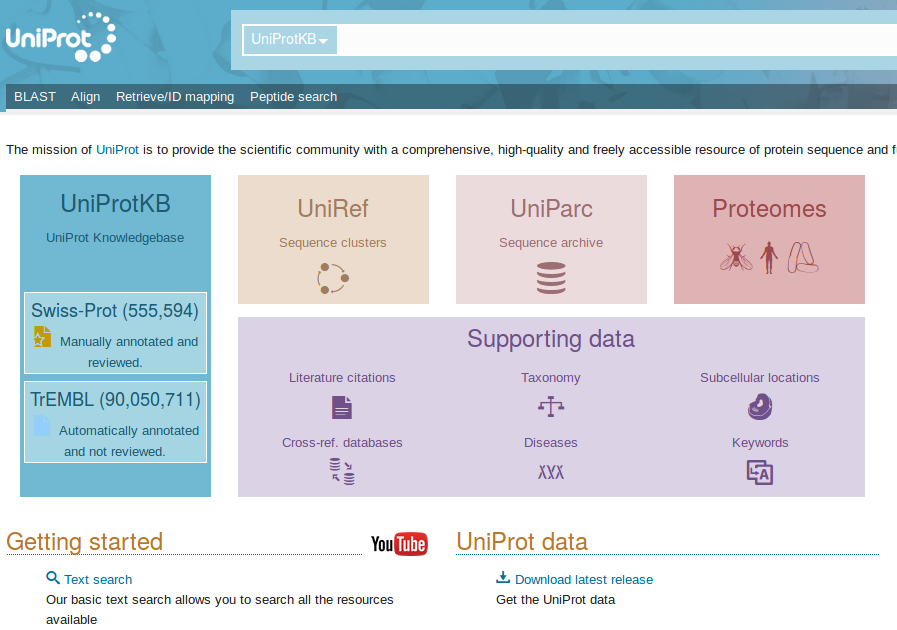
\includegraphics[width=0.8\textwidth]{./images/uniprot_main.png}
    \caption{Página principal del sitio web de UniProt.}
    \label{fig:image7}
\end{figure}

\subsection{Base de datos EROP-Moscow}

EROP-Moscow es una base de datos de secuencias de oligopéptidos de tamaño que rondan entre 2 a 50 aminoácidos altamente detalladas. Su creación se ubica en el año 1987 teniendo como autor principal a Alexander Zamyatnin y su primera publicación oficial se hizo el año 1991 \cite{erop2}. La versión de Internet de EROP-Moscow fue creada el año 2003 cuya primera publicación se hizo el año 2006 \cite{erop3}. De manera constante se le agregan nuevas secuencias investigadas \cite{eropmoscow}.

\begin{figure}[h]
    \centering
    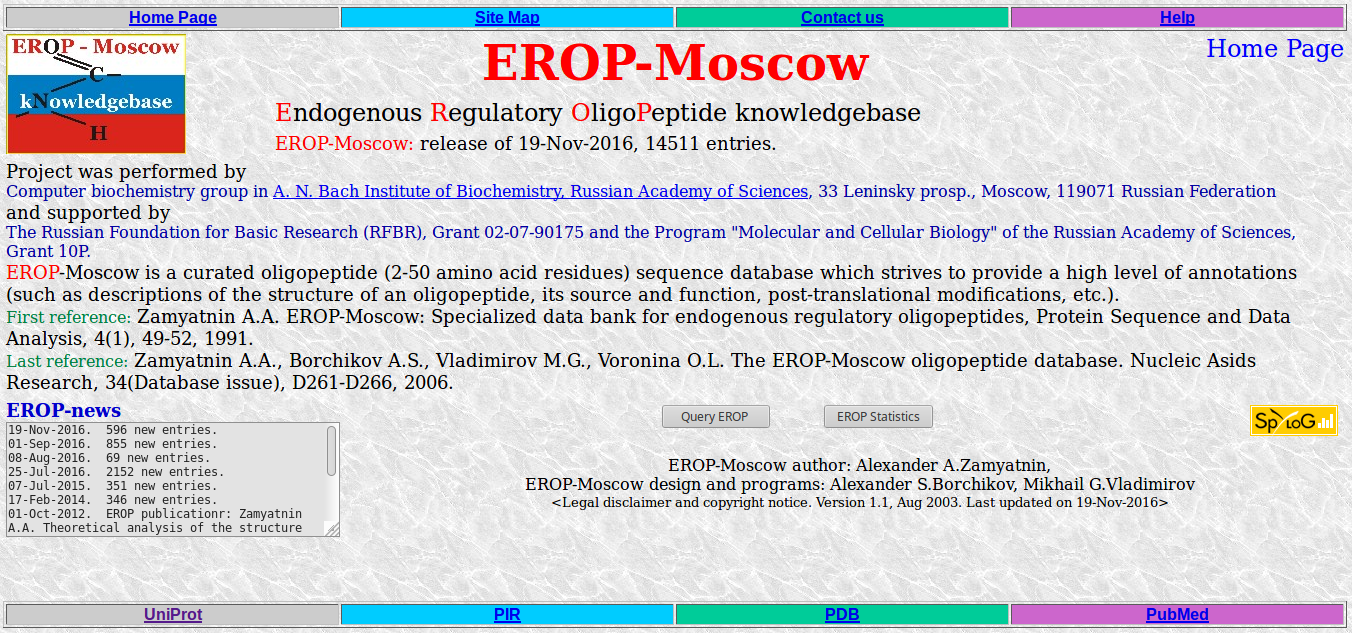
\includegraphics[width=0.8\textwidth]{./images/eropmoscow_main.png}
    \caption{Página principal del sitio web de EROP-Moscow.}
    \label{fig:image8}
\end{figure}

Actualmente está compuesta por 14.785 secuencias que equivalen a un texto con peso de 1.4 MB. Aunque son bastante pocas secuencias en comparación con UniProt, estos péptidos están descritos de manera muy completa y son ideales para realizar diferentes tipos de análisis, ya sea por sus propiedades regulatorias en los seres vivos, propiedades físico-químicas y el tipo de órgano en el cual se encuentran, entre otros.

\section{Técnicas utilizadas en el problema}

En \cite{searching} se menciona que buscar secuencias de proteínas en un predeterminado archivo (puede ser de texto o .fasta) es una tarea muy compleja, ya que se formaría un escenario similar al buscar una {\textit{aguja en un pajar}} y recorrer millones de secuencias en cada búsqueda no sería lo más convieniente considerando que la cantidad de proteínas que existen el día de hoy son muchas, por consiguiente una herramienta recomendable sería preprocesar la base de datos de proteínas con alguna técnica conocida o implementada. A continuación se hablará de forma general de algunos algoritmos conocidos que han tratado este problema.

\subsection{Algoritmo de fuerza bruta}

Este es el algoritmo más simple posible \cite{fuerzabruta}, ya que dado un texto de tamaño \textit{n} se revisan todas las posiciones posibles de un patrón de tamaño \textit{k $<$ n} desde el comienzo hasta el final del texto (izquierda a derecha). Para el caso puntual de los archivos .fasta es necesario extraer únicamente las cadenas de secuencias respectivas y adjuntarlas línea a línea, de esa forma es más fácil trabajarlas. Luego, y siguiendo la teoría matemática del número máximo de fragmentos de tamaño \textit{k}, cada una de las cadenas se revisa desde la posición 0 hasta la posición \textit{n-1} (el valor de \textit{n} varía según el largo de la cadena de cada proteína) yendo de caracter a caracter un total de \textit{n-k+1} veces para cada secuencia. Lo siguiente muestra una implementación simple en lenguaje C++, acomodada para obtener los diferentes substrings de largo \textit{k} en un texto de proteínas:
\\
\begin{lstlisting}[language=C++, caption=Búsqueda utilizando fuerza bruta en C++.]
set <string> unicos;
ifstream proteinas("proteinas.txt"); //nombre generico
string secuencia;
for (int j = 0; j < cantidad_ss; j++)
{
    getline(proteinas, secuencia);
    int n = secuencia.size();
    int maximo = n-k+1; // k entre 1 a 50
    for (int i = 0; i < maximo; i++)
    {
        string pruebas = secuencia.substr(i,k);
        if (pruebas.find_first_of("BOUXZ")==std::string::npos)
        {
            unicos.insert(pruebas);
        }
    }
}
cout << unicos.size() << endl;
\end{lstlisting}

Resumiendo, el algoritmo agrega TODOS los substrings de tamaño \textit{k} que encuentra en un string, moviéndose caracter por caracter y se verifica si el substring no posee algún aminoácido que no se encuentre dentro de los 20 aa. mencionados anteriormente. En caso afirmativo el substring se ingresa al set, estructura cuya cualidad es no repetir elementos en su conjunto. Una vez realizado todo esto, se puede obtener el número de diferentes substrings de tamaño $k$ que se encuentran en el texto, que es la gran ventaja que posee esta implementación, por lo que puede servir como un ``verificador de resultados'' cuando se analicen los resultados de implementaciones más óptimas.

Como desventajas importantes resalta el hecho de que el tiempo de ejecución es muy alto. La complejidad es de $O(n-k+1)$ por cadena, si se tiene que $N$ es la cantidad total de proteínas la complejidad en el texto sería de $O(N(n-k+1))$. Esto es linealmente afectado por el tamaño del texto a trabajar: usar un texto de 40 GB como ``uniprot\_trembl.fasta'', tomaría casi 20 horas en obtener los diferentes substrings para \textit{k = 15}). Además para almacenar un \texttt{set$<$string$>$} en C++ requiere de una gran capacidad de memoria RAM, la cual va en aumento si \textit{k} crece su valor. Por otra parte esta implementación tampoco entrega la factibilidad de encontrar una manera de extraer aquellos substrings de tamaño $k$ que más se repiten. Por consiguiente esta implementación básica no ayuda a realizar por completo la tarea esperada para este trabajo. 


\subsection{Algoritmos de búsqueda de strings}

Esta clase de algoritmos (en inglés conocidos como \textit{string searching algorithm}) tratan de localizar si uno o varios strings solicitados (llamados patrones) aparecen en un string más largo. En la mayoría de las ocasiones este alfabeto ($\Sigma$) es el que determina el rendimiento de determinado algoritmo (una variación de este alfabeto puede ayudar o perjudicar la eficiencia de un algoritmo en particular), como también el texto a analizar.
Una clasificación básica de estos algoritmos se puede realizar según la cantidad de strings a encontrar:
\begin{enumerate}
\item Algoritmos de búsqueda de un único patrón (\textit{Single pattern algorithms})
\item Algoritmos de búsqueda de múltiples patrones (\textit{Multiple pattern algorithms})
\end{enumerate}

\subsubsection{Algoritmos de búsqueda de un único patrón}

Esta clase de algoritmo de búsqueda consiste en encontrar las ocurrencias de un determinado patrón \cite{stringmatching} $p=p_{1}p_{2}$ $\ldots$ $p_{m}$ en un texto largo $T=T_{1}T_{2}$ $\ldots$ $T_{n}$, donde $p$ y $T$ son secuencias de caracteres que provienen de set finito de caracteres $\Sigma$.
Para este caso se describirán de manera sencilla los algoritmos más reconocidos que han sido desarrollados para este problema, que son el algoritmo de \textbf{Knuth-Morris-Pratt} y el algoritmo de \textbf{Boyer-Moore}.

$a)$ \textbf{Algoritmo de Knuth-Morris-Pratt}

Este algoritmo desarrollado el año 1977 por Donald E. Knuth, James H. Morris, y Vaughan R. Pratt busca como objetivo minimizar la cantidad de comparaciones del patrón \textit{p} con el texto \textit{T} manteniendo una pista de información obtenida en informaciones previas, valiéndose de la ayuda de una función de fallo (preproceso del patrón) que indica cuando la última comparación se puede reusar si existe un fallo (revisar \cite{knuthmorrispratt} para mayores detalles). Las comparaciones de caracteres se realizan de izquierda a derecha buscando el prefijo más largo posible y usarlo como información importante en las iteraciones siguientes (pseudocódigo en sección Apéndice, algoritmo \ref{alg:algoritmo1}). Se puede tomar como ejemplo el texto ``aaaabaabaaab'' y el patrón ``aabaaa''.
\\
\begin{table}[h]
\centering
\label{my-label6}
\begin{tabular}{lllllllllllll}
\cline{2-13}
\multicolumn{1}{l|}{T:} & \multicolumn{1}{l|}{a} & \multicolumn{1}{l|}{a} & \multicolumn{1}{l|}{a}                         & \multicolumn{1}{l|}{a}                         & \multicolumn{1}{l|}{b} & \multicolumn{1}{l|}{a}                         & \multicolumn{1}{l|}{a}                         & \multicolumn{1}{l|}{b}                         & \multicolumn{1}{l|}{a}                         & \multicolumn{1}{l|}{a}                         & \multicolumn{1}{l|}{a}                         & \multicolumn{1}{l|}{b} \\ \cline{2-13} 
\multicolumn{1}{l}{P1:}   & \multicolumn{1}{l}{a} & \multicolumn{1}{l}{a} & \multicolumn{1}{l}{\cellcolor[HTML]{FD6864}b} &                                                &                        &                                                &                                                &                                                &                                                &                                                &                                                &                        \\ 
P2:               & \multicolumn{1}{l}{}  & \multicolumn{1}{l}{a} & \multicolumn{1}{l}{a}                         & \multicolumn{1}{l}{\cellcolor[HTML]{FD6864}b} &                        &                                                &                                                &                                                &                                                &                                                &                                                &                        \\
  P3:                      &                        & \multicolumn{1}{l}{}  & \multicolumn{1}{l}{a}                         & \multicolumn{1}{l}{a}                         & \multicolumn{1}{l}{b} & \multicolumn{1}{l}{a}                         & \multicolumn{1}{l}{a}                         & \multicolumn{1}{l}{\cellcolor[HTML]{FD6864}a} &                                                &                                                &                                                &                        \\
 P4:                    &                        &                        &                                                &                                                & \multicolumn{1}{l}{}  & \multicolumn{1}{l}{\cellcolor[HTML]{9AFF99}a} & \multicolumn{1}{l}{\cellcolor[HTML]{9AFF99}a} & \multicolumn{1}{l}{\cellcolor[HTML]{9AFF99}b} & \multicolumn{1}{l}{\cellcolor[HTML]{9AFF99}a} & \multicolumn{1}{l}{\cellcolor[HTML]{9AFF99}a} & \multicolumn{1}{l}{\cellcolor[HTML]{9AFF99}b} &                        \\        
\end{tabular}
\caption{Ejemplo de uso del algoritmo de Knuth-Morris-Pratt.}
\end{table}

Apreciando la imagen se puede identificar que el algoritmo KMP realiza un total de 14 comparaciones hasta encontrar que el patrón aparece en el texto, en el caso de la fuerza bruta hubiesen sido necesarias 21 comparaciones hasta identificar que el patrón está en el texto.
El tiempo de preprocesamiento del texto va del orden $O(m)$ donde $m$ es el largo del patrón, y el tiempo que demora el patrón en ser ubicado en el texto es aproximadamente del orden $O(n)$ donde $n$ es el largo del texto.

$b)$ \textbf{Algoritmo de Boyer-Moore}

Este algoritmo desarrollado por Bob Boyer y J. Strother Moore el año 1977 se desmarca del algoritmo KMP ya que para Boyer-Moore se realiza la comparación entre patrón y texto de derecha a izquierda, por ejemplo si hubiera una discrepancia en el último carácter del patrón y el carácter del texto no aparece en todo el patrón, entonces éste se puede deslizar $m$ posiciones sin realizar ninguna comparación extra. En particular, no es necesario comparar los primeros $m-1$ caracteres del texto, lo cual indica que podría realizarse una búsqueda en el texto con menos de $n$ comparaciones; sin embargo, si el carácter discrepante del texto se encuentra dentro del patrón, éste podría desplazarse en un número menor de espacios \cite{boyermoore}. Esto le entrega una gran ventaja de tiempo y espacio en comparación al algoritmo KMP, en especial cuando el patrón analizado es grande (compuesto por más de 10 caracteres). Para ello se vale de la ayuda de un preprocesamiento del patrón para obtener la posición de ocurrencia de cada uno de los diferentes caracteres involucrados y un localizador de sufijos (pseudocódigo en sección Apéndice, algoritmo \ref{alg:algoritmo2}). Ahora bien, volviendo a realizar la comparación tomando el texto ``aaaabaabaaab'' y el patrón ``aabaaa'': 

\begin{table}[h]
\centering
\label{my-label7}
\begin{tabular}{lllllllllllll}
\cline{2-13}
\multicolumn{1}{l|}{T:}  & \multicolumn{1}{l|}{a}                         & \multicolumn{1}{l|}{a}                         & \multicolumn{1}{l|}{a}                         & \multicolumn{1}{l|}{a}                         & \multicolumn{1}{l|}{b}                         & \multicolumn{1}{l|}{a}                         & \multicolumn{1}{l|}{a}                         & \multicolumn{1}{l|}{b}                         & \multicolumn{1}{l|}{a}                         & \multicolumn{1}{l|}{a}                         & \multicolumn{1}{l|}{a}                         & \multicolumn{1}{l|}{b} \\ \cline{2-13} 
\multicolumn{1}{l}{P1:} & \multicolumn{1}{l}{a} & \multicolumn{1}{l}{a} & \multicolumn{1}{l}{b} & \multicolumn{1}{l}{a} & \multicolumn{1}{l}{\cellcolor[HTML]{FD6864}a} & \multicolumn{1}{l}{\cellcolor[HTML]{9AFF99}a} &                    &       &                       &        &                       &                        \\
P2:                      &                       &  & \multicolumn{1}{l}{a} & \multicolumn{1}{l}{a} & \multicolumn{1}{l}{b} & \multicolumn{1}{l}{a} & \multicolumn{1}{l}{a} & \multicolumn{1}{l}{\cellcolor[HTML]{FD6864}a} &              &               &                     &                        \\
P3:                      &                       &                       &                        &                      &  & \multicolumn{1}{l}{\cellcolor[HTML]{9AFF99}a} & \multicolumn{1}{l}{\cellcolor[HTML]{9AFF99}a} & \multicolumn{1}{l}{\cellcolor[HTML]{9AFF99}b} & \multicolumn{1}{l}{\cellcolor[HTML]{9AFF99}a} & \multicolumn{1}{l}{\cellcolor[HTML]{9AFF99}a} & \multicolumn{1}{l}{\cellcolor[HTML]{9AFF99}a} &                        \\
\end{tabular}
\caption{Ejemplo de uso del algoritmo de Boyer-Moore.}
\end{table}

Para este ejemplo se puede apreciar que con Boyer-Moore se realizan 9 comparaciones totales hasta finalmente encontrar que el patrón está ubicado en el texto, mejorando el resultado de Knuth-Morris-Pratt.
Este algoritmo tiene un tiempo de preprocesamiento del orden de $O(m+k)$ donde $m$ es el largo del patrón y $k$ es cantidad de elementos que componen el alfabeto utilizado; el tiempo que demora en encontrar el patrón en el texto varía entre el orden $O(n/m)$ para el mejor caso y el orden $O(nm)$ para el peor caso, considerando $n$ como el largo del texto en cuestión.

Mirando de una visión macro, pareciera ser que estos algoritmos tuvieran un mejor comportamiento a nivel de tiempo y rendimiento que el algoritmo de fuerza bruta, ¿pero son realmente convenientes para aplicarlos a archivos grandes de proteínas en formatos .fasta? Por una parte, estos algoritmos requieren de un \textbf{patrón}, que en este caso serían los posibles residuos de aminoácidos que existen para un tamaño $k$, por consiguiente, hay que ponerse en el caso de que se buscan los diferentes residuos de proteínas de largo 6, que equivalen a comparar las 64.000.000 combinaciones posibles y buscarlas en el archivo, que si es grande (por ejemplo superior a los 100 MB) demoraría mucho tiempo porque en ciertos casos podría ocurrir de que se revise para un solo residuo todo el archivo y no encontrarlo en el texto, en consecuencia revisar a cada rato el archivo desde el principio es un objetivo que se desea evitar para este caso del trabajo.

Casi 40 años han pasado desde que estos 2 algoritmos aparecieron para trabajarlos, sin embargo y con el paso del tiempo han aparecido nuevas mejoras de estas implementaciones (como Horsepool) o simplemente nuevos algoritmos que utilizan acercamientos en base a factores intermedios (como el algoritmo BOM - \textit{Backward Oracle Matching}), aunque estas nuevas implementaciones también caen en lo mismo, volver a utilizar como patrones a todos los potenciales residuos de aminoácidos de largo \textit{k}, y usando valores de \textit{k} muy largos puede ser una tarea infinita de realizar.

\subsubsection{Algoritmos de búsqueda de múltiples patrones}

Esta clase de algoritmos es una extensión del punto anterior, ya que aquí se buscan de manera simultánea si un conjunto de patrones $P=$\{$p_{1}$, $p_{2}$, $\ldots$, $p_{3}$\} aparece en un texto $T$ dado un set de caracteres $\Sigma$ \cite{stringmatching}. Las implementaciones más reconocidas para este caso son el algoritmo de \textbf{Aho-Corsack} (una extensión de algoritmo de Knuth-Morris-Pratt), el algoritmo de \textbf{Commentz-Walter} (una extensión del algoritmo de Boyer-Moore) y el algoritmo de \textbf{Set-BOM} (una extensión del algoritmo \textit{Backward Oracle Matching}). 

Como es lógico, aumentar la cantidad de palabras (patrones) a comparar en el texto determinado toma un proceso más caro a nivel de espacio, pero considerando que se tuviera un gran rango de patrones a buscar, como el caso de todos los potenciales péptidos de tamaño $k$ a encontrar, tomaría una visión mucho más optimista que usando un algoritmo de búsqueda con un solo patrón incluyendo una optimización en los tiempos totales de búsqueda. No obstante, se repetiría el mismo fenómeno con los archivos de gran tamaño, requiriendo de un patrón para localizar y que puede no estar en el texto, lo que supondría un gasto de tiempo innecesario e infructuoso para este trabajo, si esto se traduce en tener muchos substrings para analizarlos como patrones en este caso, por consiguiente utilizar estos algoritmos no es conveniente.



\subsection{Estructuras de datos para texto}

Los casos vistos anteriormente tienen como principal problema que para cada patrón dado, es necesario \textbf{revisar el texto desde el inicio hasta llegar a la ubicación donde el patrón existe o simplemente recorrer el texto completo sin ubicar al patrón}, ejemplificando, sería como tener que llevar 20 ovejas de La Serena a Santiago y se va trasladando de una a una generando una pérdida inmensa de tiempo y costo, por ende tiene mucho más sentido agrupar estas ovejas y luego llevarlas todas juntas a su destino. Por lo tanto lo que se busca en definitiva es \textbf{organizar todos los patrones en una única estructura de datos}, y para lograr esta tarea, no será necesario tener a mano a los patrones a buscar, sino que al \textbf{texto en sí} el cual puede ser agrupado como una larga ``cadena de strings''.

Llevando a un ejemplo más concreto y sencillo, se tiene la palabra MISSISSIPPI\$ que está compuesta por 12 letras o caracteres. Cada caracter se podría representar por medio de un índice (indexar la palabra) y quedaría de la siguiente forma:

\begin{table}[h]
\centering
\begin{tabular}{llllllllllll}
0                       & 1                      & 2                      & 3                      & 4                      & 5                      & 6                      & 7                      & 8                      & 9                      & 10                     & 11                     \\ \hline
\multicolumn{1}{|l|}{M} & \multicolumn{1}{l|}{I} & \multicolumn{1}{l|}{S} & \multicolumn{1}{l|}{S} & \multicolumn{1}{l|}{I} & \multicolumn{1}{l|}{S} & \multicolumn{1}{l|}{S} & \multicolumn{1}{l|}{I} & \multicolumn{1}{l|}{P} & \multicolumn{1}{l|}{P} & \multicolumn{1}{l|}{I} & \multicolumn{1}{l|}{\$} \\ \hline
\end{tabular}
\caption{Índices de la palabra MISSISSIPPI\$.}
\end{table}

El concepto \textbf{sufijo} corresponde para este contexto al sector de la palabra desde un punto medio (que puede ser incluso el comienzo de la palabra) hasta el final (el prefijo recurre un sector desde el inicio hasta el punto intermedio), lo cual será útil para el siguiente punto.
A partir de la imagen superior es posible obtener los ``sufijos'' de esta palabra, para posteriormente agrupar todos estos ``sufijos'' e ir ordenándolos alfabéticamente (observar Tabla 2.8 en la siguiente página).

\begin{table}[h]
	\centering
	\label{my-label8}
	\begin{tabular}{c l c c l}
		0 & MISSISSIPPI\$ &  & 11 & \$\\
		1 & ISSISSIPPI\$ &  & 10 & I\$\\
		2 & SSISSIPPI\$ &  & 7 & IPPI\$\\
		3 & SISSIPPI\$ &  & 4 & ISSIPPI\$\\
		4 & ISSIPPI\$ &  & 1 & ISSISSIPPI\$\\
		5 & SSIPPI\$ &  & 0 & MISSISSIPPI\$\\
		6 & SIPPI\$ &  & 9 & PI\$\\
		7 & IPPI\$ &  & 8 & PPI\$\\
		8 & PPI\$ &  & 6 & SIPPI\$\\
		9 & PI\$ &  & 3 & SISSIPPI\$\\
		10 & I\$ &  & 5 & SSIPPI\$\\
		11 & \$ &  & 2 & SSISSIPPI\$\\
	\end{tabular}
\caption{Sufijos (sector izquierdo) e índices (sector derecho) ordenados según orden alfabético.}
\end{table}

La clave de este ordenamiento está en el \textbf{nuevo orden que tienen los índices}, los cuales tendrán una vital importancia a la hora del desarrollo de esta memoria, y que pueden ser implementados a partir de la palabra o texto entregado para luego guardarlos y registrarlos en un vector.

Los algoritmos encargados de trabajar con este tipo de indexación son conocidos como \textbf{Búsqueda de Datos Indexados} (en inglés se conocen como \textit{Indexed Text Searching}) y de los cuales se describirán los más conocidos.

\subsection{Árbol de sufijos}

Para la lectura de las secuencias de proteínas y ADN, actualmente se considera el uso de los árboles de sufijos \cite{pekka} o también conocido como el \textit{suffix tree}, el cual es muy usado para leer cadenas de strings, ya que es ideal para desarrollar diversos problemas relativos al uso de strings como hallar substrings en común, comparación de estadísticas, proyectos relacionados con el genoma, entre otros. \\
Formalmente hablando, el árbol de sufijos \cite{sufijos} es una estructura de datos comprimida que sirve para almacenar una cadena de caracteres con “información pre-procesada” sobre su estructura interna. Según lo definió Weiner en 1973 \cite{pavesi} el árbol de sufijos $\tau$ para un string $S$ de largo $m=s_{1}s_{2}...s_{m}$ posee un nodo de inicio, y nodos hoja o hijos (que serán al menos 2). Comienza leyendo $s_{1}$, luego lee $s_{2}$ (que es $s_{1}$ quitándole la primera letra respectiva desde izquierda a derecha) identificando si hay strings que ya formaron una descendencia similar para continuar por la hoja y no crear otra y en caso contrario crear una nueva hoja, hasta así leer todo el string. En ciertas oportunidades, un sufijo de $S$ podría coincidir con el prefijo de algún otro sufijo de $S$, por lo tanto el camino para el primer sufijo no terminaría en una hoja. Por ello que la solución creada fue añadir un carácter terminador, siendo usado comúnmente el $\$$ para este caso.
\\Esto es muy útil, por ejemplo, para resolver el problema de la subcadena en tiempo lineal ya que se tiene este texto $S$ de longitud $m$ el cual se pre-procesa (se construye el árbol) en tiempo de orden $O(m)$ donde se busca una subcadena $P$ de longitud $n$ (cuyo tiempo es de $O(n)$).

\begin{figure}[h]

\begin{subfigure}{0.5\textwidth}
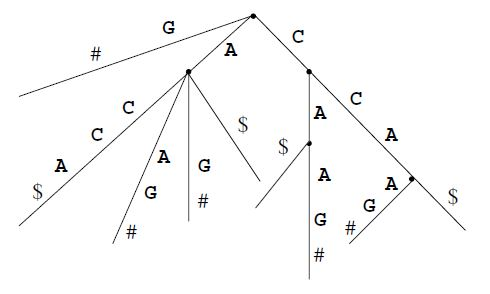
\includegraphics[width=0.9\linewidth, height=5cm]{./images/suffixtree1.JPG} 
\caption{Árbol de sufijos de una cadena de ADN aleatoria.}
\label{fig:subim5}
\end{subfigure}
\begin{subfigure}{0.5\textwidth}
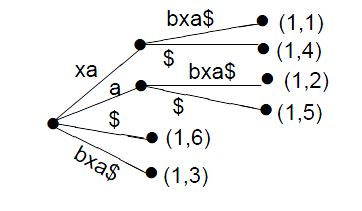
\includegraphics[width=0.9\linewidth, height=5cm]{./images/suffixtree2.JPG}
\caption{Árbol de sufijos de la palabra $xabxa$.}
\label{fig:subim6}
\end{subfigure}
 
\caption{Ejemplos de árboles de sufijos.}
\label{fig:image3}
\end{figure}

El problema para la secuencia de ADN considera que habrá un conjunto de textos $S_{i}$ pertenecientes a la cadena de nucleóticos, y en el cual poder verificar si $P$ es subcadena de algún $S_{i}$, lo que es llamado {\it{el árbol de sufijos generalizado}} (ver Figura \ref{fig:mesh1}). 

\begin{figure}[h]
    \centering
    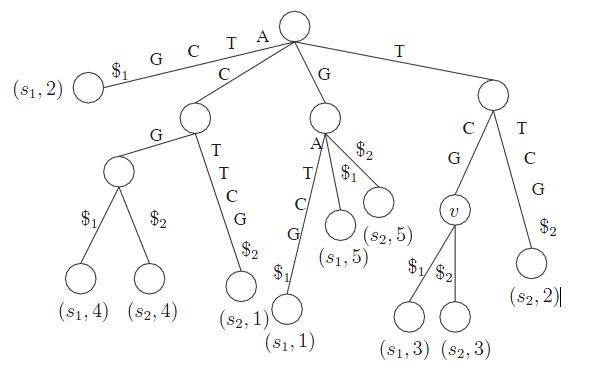
\includegraphics[width=0.55\textwidth]{./images/suffixtree3.JPG}
    \caption{El árbol de sufijo generalizado para las secuencias {\it{GATCG\$}} y {\it{CTTCG\$}} \cite{koaluru}.}
    \label{fig:mesh1}
\end{figure}

\subsection{Arreglo de sufijos}

Los arreglos de sufijos fueron introducidos por Udi Mander y Gene Myers el año 1990 \cite{suffixarray1} y corresponden a una variante del árbol de sufijos mucho más eficiente en cuanto al uso de la memoria \cite{licenciado}. 

Hablando de manera más formal, sea $T=t_{1}, t_{2},$ $\ldots$ $,t_{n}$ una cadena y sea $T[i,j]$ la subcadena que va del índice $i$ hasta $j$. El arreglo de sufijos $SA$ de la cadena $T$ va a ser un arreglo de enteros brindando las posiciones iniciales de los sufijos en $T$ en órden lexicográfico. Esto significa que $SA[i]$ contiene la posicion inicial del $i$-ésimo sufijo más pequeño en $T$ y por tanto se cumple que para todo $1 < i \leq n: T[SA[i-1],n] < T[SA[i],n]$. 

Reutilizando el ejemplo de la palabra MISSISSIPPI\$, el arreglo de sufijos que contiene las posiciones iniciales sería el siguiente:

\begin{table}[h]
\centering
\label{my-label9}
\begin{tabular}{|
>{\columncolor[HTML]{EFEFEF}}c|c|c|c|c|c|c|c|c|c|c|c|c|}
\hline
$i$        & 0  & 1  & 2 & 3 & 4 & 5 & 6 & 7 & 8 & 9 & 10 & 11 \\ \hline
$SA{[}i{]}$ & 11 & 10 & 7 & 4 & 1 & 0 & 9 & 8 & 6 & 3 & 5  & 2  \\ \hline
\end{tabular}
\caption{Arreglo de sufijos $A[i]$ de la palabra MISSISSIPPI\$.}
\end{table} 

Para este tipo de estructura, y tal como menciona \cite{abeliuk}, encontrar un patrón $P$ de tamaño $m$ (donde $m < n$) en el texto consiste en buscar el intervalo $[j,k]$ en el arreglo que contiene a todos los sufijos que comienzan con el patrón mencionado. Esto se logra mediante una búsqueda binaria sobre $A$, buscando lexicográficamente el menor sufijo que parte con $P$, y otra búsqueda binaria buscando el mayor sufijo que parte con $P$. En cada comparación de esta búsqueda binaria se compara un sufijo con el patrón, lo que toma tiempo $O(m)$ en el peor caso, luego la búsqueda completa toma $O(m \log n)$. Junto con el arreglo de sufijos es necesario guardar el texto, y ambos juntos ocupan $O(n \log n)$ bits de espacio y un tiempo del orden de $O(n (\log n)^{2})$ \cite{suffixarray2} (pseudocódigo en sección Apéndice, algoritmo \ref{alg:algoritmo3}).

\subsubsection*{Diferencias entre árbol de sufijos y arreglo de sufijos}

Ambas estructuras representan (entregan como salida) el mismo resultado, pero con varias discrepancias. La más obvia, es que el \textit{suffix tree} es un árbol donde al recorrer cada una de sus hojas se obtiene el arreglo de sufijos. No obstante, la diferencia importante entre ambos algoritmos radica en \textbf{la cantidad de espacio utilizada}. La construcción del árbol de sufijos toma tiempo lineal en el largo del texto. El árbol de sufijos tiene $O(n)$ nodos. Luego, dado que los substrings de cada rama pueden ser guardados como la posición y el largo de un substring del texto $S$, un árbol de sufijos de $n$ nodos ocupa $O(n \log n)$ bits. Esto permite realizar varias operaciones sobre los nodos del \textit{suffix tree}. Sin embargo esto se convierte en un problema porque implica un tamaño de almacenamiento de varias veces el texto original \cite{abeliuk}. 

Por el contrario el arreglo de sufijos pierde varias de estas funciones a cambio de una importante mejora en cuanto a los requerimientos en espacio de los árboles de sufijos porque el \textit{suffix array} guarda \textbf{$n$ enteros}. Por lo cual si se tiene un arreglo donde un entero requiere 4 $bytes$ (32 bits), un arreglo de sufijos en ese caso requeriría un total de implementación de $4n$ $bytes$ (si el entero necesitara 8 $bytes$ (64 bits), el arreglo tendría un tamaño de $8n$ $bytes$). Y esto es significativamente menor que los $20n$ bytes requeridos en la implementación del árbol de sufijos \cite{kurtz}.

\subsection{Arreglo LCP}

LCP es una sigla en inglés que hace referencia al ``Prefijo común más largo'' (LCP = \textit{Longest Common Prefix}). Este arreglo es una estructura auxiliar al arreglo de sufijos (tamaño igual al del \textit{suffix array}), pero que en sus posiciones guarda las longitudes de los prefijos comunes más largos entre todos los pares de sufijos consecutivos correspondientes al arreglo de sufijos. 

Esta estructura fue introducida el año 1990 por Udi Manber y Gene Myers con la finalidad de optimizar el tiempo de ejecución para la búsqueda de strings \cite{suffixarray1}. Y de manera formal se define como: Se tiene $SA$ que es el arreglo de sufijos del texto $T=t_{0}t_{1}$ $\ldots$ $t_{n-1}$ y $lcp(v,w)$ es el largo del prefijo común más largo entre 2 strings $v$ y $w$. Además se sabe que $T[i,j]$ es el substring de $S$ que va desde la posición $i$ hasta $j$. Por consiguiente el arreglo $LCP[0,n-1]$ es un arreglo compuesto de números enteros de tamaño $n$ donde $LCP[0]$ está indefinido y $LCP[i] = lcp(T[SA[i-1],n], T[SA[i],n])$ para todo $1 < i \leq n$. Por consiguiente $LCP[i]$ almacena la longitud del prefijo común más largo del -lexicográficamente hablando-  $i$-ésimo sufijo más pequeño y su predecesor en el \textit{suffix array}.

Para mostrar un ejemplo, se usará nuevamente la palabra MISSISSIPPI\$ en base al SA obtenido anteriormente, mostrando también sus sufijos ordenados (ver Tabla 2.11). A partir de esto el arreglo LCP es construido comparando lexicográficamente a los sufijos consecutivos para determinar el prefijo común más largo (ver Tabla 2.12).

\begin{table}[!htb]
\centering
\label{my-label10}
\begin{tabular}{|l|l|l|l|l|l|l|l|l|l|l|l|l|}
\hline
\textbf{i}         & \multicolumn{1}{c|}{0}  & \multicolumn{1}{c|}{1}  & \multicolumn{1}{c|}{2} & \multicolumn{1}{c|}{3} & \multicolumn{1}{c|}{4} & \multicolumn{1}{c|}{5} & \multicolumn{1}{c|}{6} & \multicolumn{1}{c|}{7} & \multicolumn{1}{c|}{8} & \multicolumn{1}{c|}{9} & \multicolumn{1}{c|}{10} & \multicolumn{1}{c|}{11} \\ \hline
\textbf{T{[}i{]}}  & \multicolumn{1}{c|}{m}  & \multicolumn{1}{c|}{i}  & \multicolumn{1}{c|}{s} & \multicolumn{1}{c|}{s} & \multicolumn{1}{c|}{i} & \multicolumn{1}{c|}{s} & \multicolumn{1}{c|}{s} & \multicolumn{1}{c|}{i} & \multicolumn{1}{c|}{p} & \multicolumn{1}{c|}{p} & \multicolumn{1}{c|}{i}  & \multicolumn{1}{c|}{\$}  \\ \hline
\textbf{SA{[}i{]}} & \multicolumn{1}{c|}{11} & \multicolumn{1}{c|}{10} & \multicolumn{1}{c|}{7} & \multicolumn{1}{c|}{4} & \multicolumn{1}{c|}{1} & \multicolumn{1}{c|}{0} & \multicolumn{1}{c|}{9} & \multicolumn{1}{c|}{8} & \multicolumn{1}{c|}{6} & \multicolumn{1}{c|}{3} & \multicolumn{1}{c|}{5}  & \multicolumn{1}{c|}{2}  \\ \hline
\textbf{0}                                                       & \$                       & i                       & i                      & i                      & i                      & m                      & p                      & p                      & s                      & s                      & s                       & s                       \\ \hline
\textbf{1}                                                       &                         & \$                       & p                      & s                      & s                      & i                      & i                      & p                      & i                      & i                      & s                       & s                       \\ \hline
\textbf{2}                                                       &                         &                         & p                      & s                      & s                      & s                      & \$                      & i                      & p                      & s                      & i                       & i                       \\ \hline
\textbf{3}                                                       &                         &                         & i                      & i                      & i                      & s                      &                        & \$                      & p                      & s                      & p                       & s                       \\ \hline
\textbf{4}                                                       &                         &                         & \$                      & p                      & s                      & i                      &                        &                        & i                      & i                      & p                       & s                       \\ \hline
\textbf{5}                                                       &                         &                         &                        & p                      & s                      & s                      &                        &                        & \$                      & p                      & i                       & i                       \\ \hline
\textbf{6}                                                       &                         &                         &                        & i                      & i                      & s                      &                        &                        &                        & p                      & \$                       & p                       \\ \hline
\textbf{7}                                                       &                         &                         &                        & \$                      & p                      & i                      &                        &                        &                        & i                      &                         & p                       \\ \hline
\textbf{8}                                                       &                         &                         &                        &                        & p                      & p                      &                        &                        &                        & \$                      &                         & i                       \\ \hline
\textbf{9}                                                       &                         &                         &                        &                        & i                      & p                      &                        &                        &                        &                        &                         & \$                       \\ \hline
\textbf{10}                                                      &                         &                         &                        &                        & \$                      & i                      &                        &                        &                        &                        &                         &                         \\ \hline
\textbf{11}                                                      &                         &                         &                        &                        &                        & \$                      &                        &                        &                        &                        &                         &                         \\ \hline
\end{tabular}
\caption{SA de MISSISSIPPI\$ y sus sufijos respectivos.}
\end{table}

Por ejemplo, $LCP[4] = 4$ que es la longitud del prefijo común más largo ISSI que se comparten entre los sufijos $SA[3] = T[4,11] =$ ISSIPPI\$ y $SA[4] = T[1,11] =$ ISSISSIPPI\$. Notar que $LCP[0] = \emptyset$ ya que no hay un sufijo más pequeño lexicográficamente hablando \cite{lcparray}.

\begin{table}[!htb]
\centering
\label{my-label11}
\begin{tabular}{|l|c|c|c|c|c|c|c|c|c|c|c|c|}
\hline
\textbf{i}         & 0  & 1  & 2 & 3 & 4 & 5 & 6 & 7 & 8 & 9 & 10 & 11 \\ \hline
\textbf{T{[}i{]}}  & m  & i  & s & s & i & s & s & i & p & p & i  & \$  \\ \hline
\textbf{SA{[}i{]}} & 11 & 10 & 7 & 4 & 1 & 0 & 9 & 8 & 6 & 3 & 5  & 2  \\ \hline
\textbf{LCP{[}i{]}} & $\emptyset$  & 0  & 1 & 1 & 4 & 0 & 0 & 1 & 0 & 2 & 1  & 3  \\ \hline
\end{tabular}
\caption{Arreglo LCP de la palabra MISSISSIPPI\$.}
\end{table}

La construcción del algoritmo del arreglo LCP se puede establecer en 2 categorías, obtener el arreglo LCP como un bi-producto del arreglo de sufijos \cite{suffixarray1} o simplemente utilizar un arreglo de sufijos previamente construído \cite{kasai}. Para este segundo caso el arreglo LCP es construido en un tiempo del orden de $O(n \log n)$, y si se asume que cada simbolo de texto pesa un byte y cada valor o elemento del arreglo de sufijos y arreglo LCP pesa 4 bytes, considerando un texto de tamaño $n$ entonces el peso total para guardar los 2 arreglos sería $8n$ (pseudocódigo en sección Apéndice, algoritmo \ref{alg:algoritmo4}).


\subsection{External Memory Suffix Array}

Como se vio anteriormente, la construcción del \textit{suffix array} (SACA, sigla en inglés de \textit{Suffix Array Construction Algorithm}) se realiza en memoria RAM, donde se almacena el texto de entrada y el posterior arreglo de sufijos. Sin embargo existen textos muy grandes como la base de datos de Wikipedia, bases de datos de genomas, variados textos que superen los 10 GB de tamaño, los cuales son tan grandes que no se podría guardar en la memoria RAM siquiera el texto en sí. Por lo mismo se ha investigado una alternativa para poder construir arreglos de sufijos para aquellos textos de gran tamaño.

Ante eso surgió el concepto del ``arreglo de sufijos en memoria externa'' (traducción en español de \textit{External Memory Suffix Array}, también es conocido como \textit{EM Suffix Array} o su abreviatura, \textit{EMSA}), que consiste en construir el arreglo de sufijos de determinado texto $T$ evitando guardar todo el texto en la memoria RAM. La idea fue introducida por Gastón Gonnet, Ricardo Baeza-Yates y Tim Snider el año 1992 \cite{newindices} y a partir de ese entonces han aparecido varias implementaciones que se diferencian en cuanto a rendimiento y tiempo (\cite{better}, \cite{esais}, \cite{sascan}).

Siguiendo lo enunciado por \cite{sascan}, la idea principal del ``arreglo de sufijos en memoria externa'' es particionar el texto en bloques que son lo suficientemente pequeños para que el arreglo de sufijos de cada bloque pueda ser construido en la memoria RAM. Entonces una vez que se tengan los arreglos de sufijos en bloques, estos se combinan formando el arreglo de sufijos completo del texto siguiendo el siguiente formato: 

\begin{figure}[!htb]
    \centering
    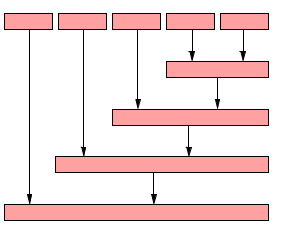
\includegraphics[width=0.6\textwidth]{./images/combinacionsascan.png}
    \caption{Arreglo de sufijos de un texto $T$ formado por la combinación de arreglos de sufijos de los bloques del texto $T$.}
    \label{fig:comb1}
\end{figure}

Se aprecia en la imagen que los bloques de \textit{suffix array} se van combinando desde el final y de manera singular, donde cada uno de ellos se va acoplando con el bloque combinado que dará como resultado al arreglo de sufijos completo para el texto $T$.

Para explicar cómo se realiza la combinación se asumirá que se tiene un string \texttt{T[0,...,n-1]} de tamaño $n$. El texto se divide en bloques de tamaño $m$, donde $m$ es elegido de tal manera que cada una de las estructuras creadas puedan ajustarse según la memoria RAM de tamaño $M$ y no sobrepasarla ($m<M$). Los bloques se procesan comenzando desde el final del texto. Suponer que hasta ahora se ha procesado \texttt{Z = T[i,...,n-1]} y a partir de ese bloque de texto se ha construído el arreglo de sufijos \texttt{SA\textsubscript{Z}}. Luego se procede a construir el arreglo de sufijos \texttt{SA\textsubscript{Y}} del bloque de texto \texttt{Y = T[i-m,...,i-1]} y combinarlo con \texttt{SA\textsubscript{Z}} para formar \texttt{SA\textsubscript{YZ}}. De manera muy general la combinación sigue 2 pasos (ver Figura \ref{fig:comb2}).

El primer paso es comparar el \textit{suffix array} de $Y$ con el texto $Z$ para formar el arreglo \texttt{gap\textsubscript{Y}} que permitirá realizar el segundo paso que es ubicar aquellos sufijos que se ubican entre \texttt{SA\textsubscript{Z}[i]} y \texttt{SA\textsubscript{Z}[i+1]} y realizar la combinación.

Como son bastantes combinaciones a realizar, la complejidad de lectura y escritura en los archivos (\textit{I/O complexity}) y bloques que se forman va por un orden proporcional de $O$($\frac{n^{2}}{M}$) y un tiempo cuya complejidad va por el orden de 0($\frac{n^{2}}{M} \log (2 + \frac{\log \rho}{\log n})$). Como se trabajará con este tipo de algoritmo para el problema de la memoria, se dará mayor detalle de su implementación en el capítulo siguiente (``Implementación'').

\begin{figure}[h]
    \centering
    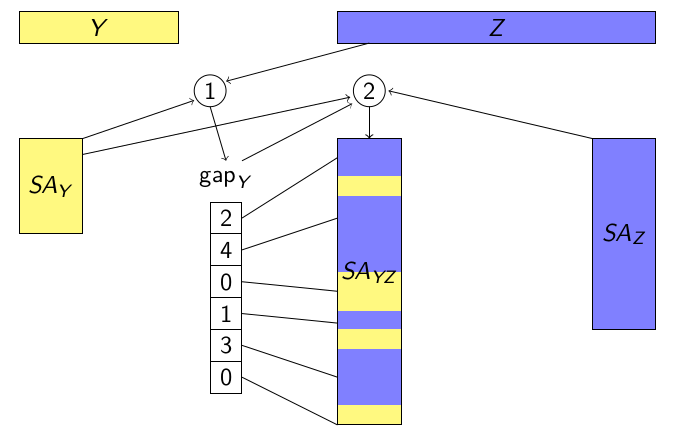
\includegraphics[width=0.8\textwidth]{./images/combinacion2bloques.png}
    \caption{Combinación de 2 arreglos de sufijos que fueron creados de los fragmentos de texto $Y$ y $Z$.}
    \label{fig:comb2}
\end{figure}

\subsection{External Memory LCP Array}

El arreglo de sufijos, en conjunto con su arreglo LCP son la base de soluciones de diversas aplicaciones \cite{aplicacion}. Por consiguiente, cuando comenzó a surgir la implementación del \textit{suffix array} en memoria externa entró a ser materia de investigación la búsqueda de la construcción de un arreglo en LCP también en memoria externa.

Como antes se mencionó, una manera optima de construir el arreglo LCP de un texto $T$ es implementando previamente el arreglo de sufijos del texto $T$ y utilizar este arreglo recien obtenido como \textit{input} para construir el arreglo LCP. Kasai \cite{kasai} fue quien pudo llevar esta idea a una implementación en memoria RAM (memoria interna) pero no fue hasta que Juha Kärkkäinen y Dominik Kempa \cite{lcpscan} pudieron desarrollar una implementación de un arreglo LCP en memoria externa usando como \textit{input} el arreglo de sufijos construido en memoria externa.

Según lo más reciente investigado \cite{emsparse} y para dar un ejemplo sencillo, para obtener el arreglo LCP en memoria externa, se tiene el siguiente texto o string \texttt{T} de tamaño $n$ (\texttt{T} = \texttt{T[0,...,n-1]} = \texttt{T[0]T[1]...T[n-1]}). A partir de este texto se obtiene su arreglo de sufijos \texttt{SA[0,...,n-1]} que es el arreglo ordenado de todos los sufijos del texto $T$. Entonces lo que se quiere obtener para todo $i$ donde $0 \leq i < n$ es el arreglo \texttt{LCP[0,...,n-1]} (el valor de \texttt{LCP[0]} es indefinido) donde \texttt{LCP[i]} = \textit{lcp(\texttt{SA[i]},\texttt{SA[i-1]})}, donde \textit{lcp(j,k)} es la longitud del prefijo común más largo entre el sufijo $j$ y $k$.

Para lograr esto se definen 2 nuevos arreglos, el \textit{arreglo $\Phi$} que consiste en que si se tiene \texttt{j = SA[i]}, entonces se cumple que \texttt{$\Phi$[j] = SA[i-1]} para todo $j$ donde $1 \leq j \leq n$. En otras palabras el sufijo $\Phi$[i] es el predecesor lexicográfico inmediato del sufijo $i$ y por lo tanto \texttt{SA[n-k] = $\Phi_{k}$[SA[n]]} $\forall$ $k$ $\in$ [0,...,n].

El segundo arreglo a definir es conocido como el \textit{arreglo LCP permutado} \texttt{PLCP[0,...,n-1]} es el arreglo LCP permutado desde el orden lexicográfico hacia el orden del texto, es decir, \texttt{PLCP[SA[j]] = LCP[j]} para todo $j$ donde $1 \leq j \leq n$. Por consiguiente \texttt{PLCP[i]} = \textit{lcp(\texttt{i},\texttt{$\Phi$[i]})} $\forall$ $i$ $\in$ [0,...,n-1]. Se considerará un ejemplo con el string \texttt{T = babaabbabbab\$}:

\begin{table}[h]
\centering
\label{my-label12}
\begin{tabular}{|r|ccccccccccccc|}
\hline
\textit{i}  & \multicolumn{1}{c|}{0} & \multicolumn{1}{c|}{1} & \multicolumn{1}{c|}{2} & \multicolumn{1}{c|}{3} & \multicolumn{1}{c|}{4} & \multicolumn{1}{c|}{5} & \multicolumn{1}{c|}{6} & \multicolumn{1}{c|}{7} & \multicolumn{1}{c|}{8} & \multicolumn{1}{c|}{9} & \multicolumn{1}{c|}{10} & \multicolumn{1}{c|}{11} & 12 \\ \hline
T{[}i{]}    & b                      & a                      & b                      & a                      & a                      & b                      & b                      & a                      & b                      & b                      & a                       & b                       & \$  \\
SA{[}i{]}   & 12                     & 3                      & 10                     & 1                      & 7                      & 4                      & 11                     & 2                      & 9                      & 0                      & 6                       & 8                       & 5  \\
$\Phi${[}i{]}  & 9                      & 10                     & 11                     & 12                     & 7                      & 8                      & 0                      & 1                      & 6                      & 2                      & 3                       & 4                       & -  \\
LCP{[}i{]}  & -                      & 0                      & 1                      & 2                      & 2                      & 5                      & 0                      & 1                      & 2                      & 3                      & 3                       & 1                       & 4  \\
PLCP{[}i{]} & 3                      & 2                      & 1                      & 0                      & 5                      & 4                      & 3                      & 2                      & 1                      & 2                      & 1                       & 0                       & -  \\ \hline
\end{tabular}
\caption{Texto \texttt{T = babaabbabbab\$} con su respectivos \texttt{SA[i]}, \texttt{$\Phi$[i]}, \texttt{LCP[i]} y \texttt{PLCP[i]}.}
\end{table}

Por ende los pasos generales para obtener el arreglo LCP en memoria externa tomando como entradas el texto $T$ y el \textit{suffix array} SA (obtenido también por memoria externa) son los siguientes:

\begin{enumerate}

\item Calcular $\Phi$ desde el SA obtenido previamente, si se da el caso se particiona el texto en bloques que se puedan ubicar en la memoria RAM.
\item Calcular el arreglo PLCP usando el arreglo $\Phi$ y el texto $T$ como base.
\item Calcular el arreglo LCP usando el arreglo PLCP obtenido, acá el texto se particiona en medio-segmentos (\textit{half-segments}) de tal manera que 2 medio-segmentos puedan ser colocados en la memoria RAM.

\end{enumerate}

Se obviarán por ahora detalles mayores de la explicación del funcionamiento de este algoritmo, ya que será analizado y profundizado en el capítulo ``Implementación'' cuando se use este algoritmo para obtener parte de los resultados de la memoria con la base de datos TrEMBL.

\subsection{Transformación de Burrows-Wheeler}

La transformación de Burrows-Wheeler \cite{bwt}, (abreviatura \textit{BWT} del inglés \textit{Burrows–Wheeler transform}, también conocida como compresión por ordenación de bloques), es un algoritmo usado en técnicas de compresión de datos. Fue inventado por Michael Burrows y David Wheeler en 1994 mientras trabajaban en el \textit{DEC Systems Research Center} en Palo Alto, California. Esta transformación consiste en que se toma un trozo de texto $T$ y se le realizan todas las rotaciones posibles, para luego ordenarlas de manera lexicográfica, obteniendo como salida la última columna ubicada en la derecha de la matriz generada (ver Figura \ref{fig:comb3}).

La aplicación más importante que tiene esta transformación es la de compresión de datos (usada por ejemplo la usada en la Alineación de Bowtie \cite{bowtie}) y también mantiene correlación con el arreglo de sufijos, el cual será utilizado en el \textit{External Memory Suffix Array} para este trabajo (en el capítulo ``Implementación'' se detallará cúal es la función de esta transformación).

\begin{figure}[h]
    \centering
    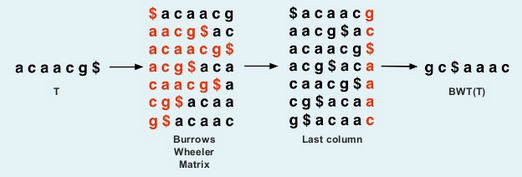
\includegraphics[width=0.6\textwidth]{./images/bwtejemplo.png}
    \caption{Ejemplo de la transformación de Burrows-Wheeler para la cadena acaacg\$.}
    \label{fig:comb3}
\end{figure}